\chapter{Methodology and Schedule} 
\epigraph{There is no greater harm than that of time wasted.}{Michelangelo}

\section{Methodology}
Tools for characterizing and analyzing performance on each specific scenario will be identified and integrated on the testing platforms. There are existing open source tools that provide the required information, but little information regarding specific use to instrument the desired scenarios.

The following are the specific scenarios that will be evaluated on each platform:
\begin{itemize*}
\item Video capture, and encoding.
\item Audio capture, and encoding.
\item Synchronized video and audio capture, encoding and storage in block-based storage device using an standard multimedia file container.
\item Synchronized video and audio capture, encoding and transmission over network using RTP/UDP/IP protocol.
\item Video decoding and preview from block-based storage device using an standard multimedia file container.
\end{itemize*}

For block-based storage device we consider any storage device with semantics similar to of standard hard disks, and specifically excluding devices based on flash memory unless they use any sort of \ac{FTL}.

The following aspects will be considered for each specific scenario:
\begin{itemize*}
\item CPU usage and scheduling overhead.
\item Memory usage and overhead by the software stack.
\item I/O usage: efficiency regarding use of the specific I/O architecture and overhead by the software stack.
\end{itemize*}

\section{Assumptions}
Describe untested and un-testable positions, basic values, world views, or beliefs that are assumed in your study.
Your examination should extend to your methodological assumptions, such as the attitude you have toward different analytic approaches and datat-gathering methods. Make the reader aware of your own biases.

\section{Procedure}
Describe in detail all the steps you will carry out to choose subjects, construct variables, develop hypotheses, gather and present data, such that another researcher could replicate your work.
Remember the presentation of data never speaks for itself, it must be interpreted.

\section{List of Deliveries}
The deliveries are:
\begin{enumerate*}
\item Patches for GStreamer to improve performance on the target scenarios and platforms.
\item Patches for the Linux kernel available for the specific platforms to improve performance.
\end{enumerate*}

As stated previously, all the patches will be designed with the intention of acceptance on their respective projects, but not guarantee is made about their merging on mainstream. Still the work will be done interacting with the respective project maintainers.

\section{Schedule and Work Breakdown}

\begin{table}[tph]
\caption{Work Breakdown} \centering
\begin{tabular}{c}
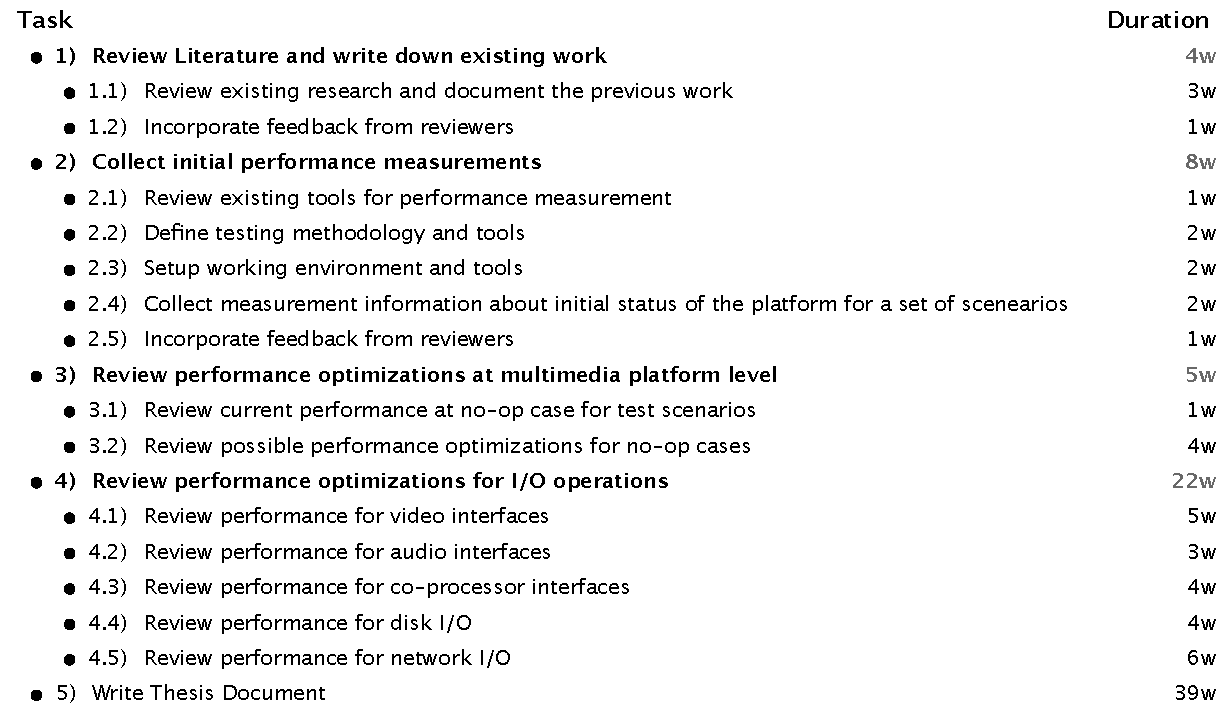
\includegraphics[width=1.0\textwidth]{images/Outline.pdf}
\end{tabular}
\end{table}

\begin{figure}[tbh]
\centering
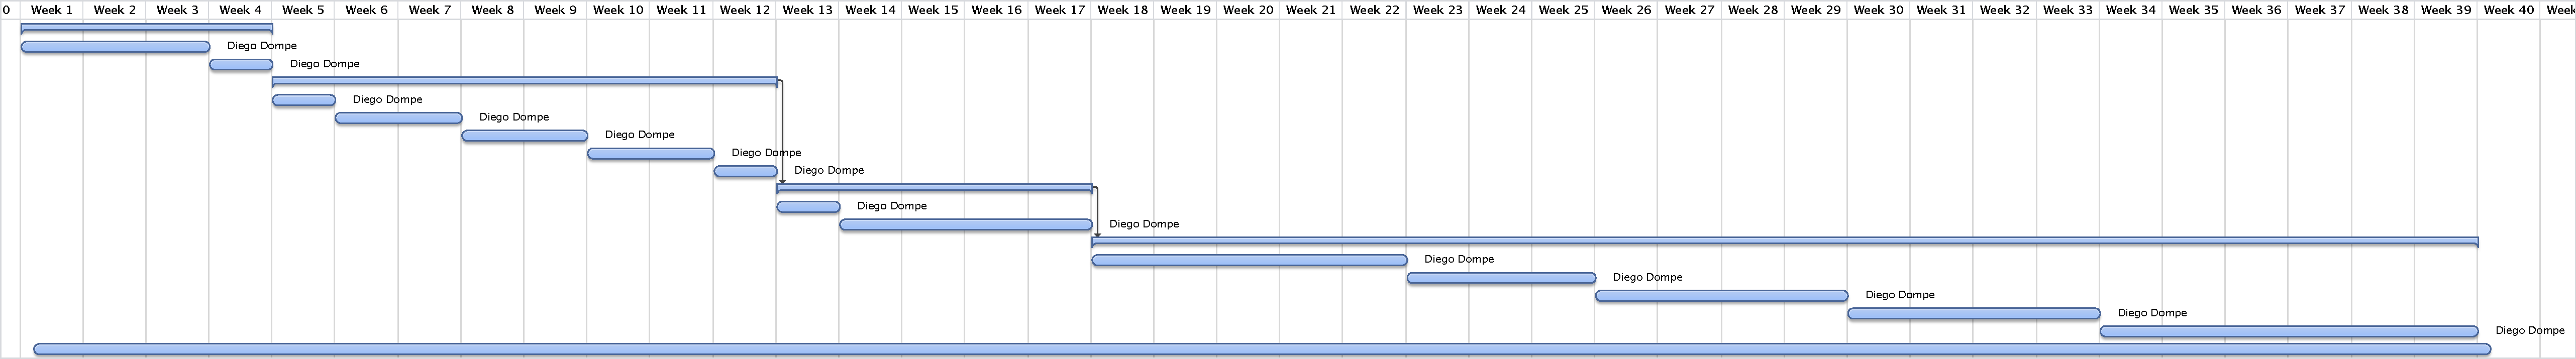
\includegraphics[width=0.55\textheight,height=0.34\textwidth,angle=90]{images/Gantt.pdf}\\
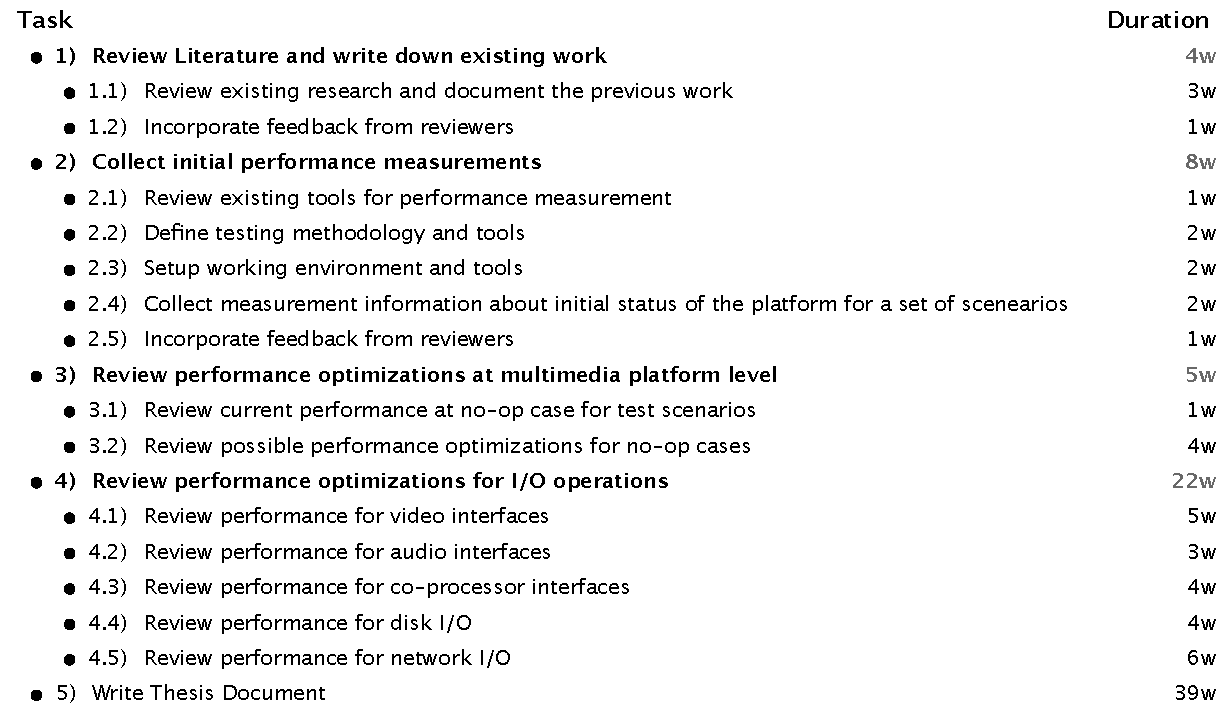
\includegraphics[width=0.4\textheight,angle=90]{images/Outline.pdf}
\caption{Gantt Chart}\label{gantt}
\end{figure}
